% \iffalse
\let\negmedspace\undefined
\let\negthickspace\undefined
\documentclass[journal,12pt,twocolumn]{IEEEtran}
\usepackage{cite}
\usepackage{amsmath,amssymb,amsfonts,amsthm}
\usepackage{algorithmic}
\usepackage{graphicx}
\usepackage{textcomp}
\usepackage{xcolor}
\usepackage{txfonts}
\usepackage{listings}
\usepackage{enumitem}
\usepackage{mathtools}
\usepackage{gensymb}
\usepackage{comment}
\usepackage[breaklinks=true]{hyperref}
\usepackage{tkz-euclide} 
\usepackage{listings}
\usepackage{gvv}                                        
\def\inputGnumericTable{}                                 
\usepackage[latin1]{inputenc}                                
\usepackage{color}                                            
\usepackage{array}                                            
\usepackage{longtable}                                       
\usepackage{calc}                                             
\usepackage{multirow}                                         
\usepackage{hhline}                                           
\usepackage{ifthen}                                           
\usepackage{lscape}
\usepackage{placeins}
\usepackage{xparse}


\newtheorem{theorem}{Theorem}[section]
\newtheorem{problem}{Problem}
\newtheorem{proposition}{Proposition}[section]
\newtheorem{lemma}{Lemma}[section]
\newtheorem{corollary}[theorem]{Corollary}
\newtheorem{example}{Example}[section]
\newtheorem{definition}[problem]{Definition}
\newcommand{\BEQA}{\begin{eqnarray}}
\newcommand{\EEQA}{\end{eqnarray}}
\newcommand{\define}{\stackrel{\triangle}{=}}
\theoremstyle{remark}
\newtheorem{rem}{Remark}

\graphicspath{ {./figs/} } 

\begin{document}

\bibliographystyle{IEEEtran}
\vspace{3cm}

\Large\title{GATE ME 30}
\large\author{EE23BTECH11032 - Kaustubh Parag Khachane $^{*}$% <-this % stops a space
}
\maketitle
\newpage
\bigskip

\renewcommand{\thefigure}{\theenumi}
\renewcommand{\thetable}{\theenumi}
\large\textbf{Question GATE ME 30} :\\
The figure shows a block of mass m = 20 kg attached to a pair of identical linear springs, each having a spring constant k = 1000 N/m. The block oscillates on a frictionless horizontal surface. Assuming free vibrations, the time taken by the block to complete ten oscillations is \rule{1cm}{0.15mm} seconds . (Rounded off to two decimal places) Take $\pi$ = 3.14. \\ \hfill(GATE ME 2023)

\begin{figure}[!ht]
\centering
\begin{center}
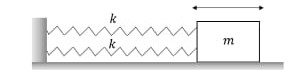
\includegraphics[width=\columnwidth]{questiondiagram}
\end{center}
%\caption{Diagram for GATE ME Question 30}
\end{figure}

\solution\\
\begin{table}[!ht] 
\centering
\setlength{\extrarowheight}{8pt}
\begin{tabular}{|l|l|l|}
    \hline
    \textbf{Parameter} & \textbf{Description} & \textbf{Value} \\
    \hline
     m & Mass of object & 10 Kg \\\hline
     $\mu$ & Frictional coefficient \brak{static} & 0.25\\\hline
     x\brak{t} & Displacement of block &  \\\hline
     $x\brak{0}$ & Initial displacement & 0 \brak{assumed} \\\hline
     g & Gravitational acceleration & 10 $m/s^2$ \\\hline
     $F_s$ & Spring force &  \\\hline
     f & frictional force &  $\mu$ N \\\hline
     N & Normal Force & mg $cos\brak{\theta}$ \\\hline
    \end{tabular}
  \vspace{4mm}
 \caption{Parameter Table}
 \label{tab:table0_xe80}
\end{table}

\begin{align}
    F &= ma \\
    F &= -kx \\
    \implies ma + kx &= 0\\
    \therefore m\frac{d^2x}{dt^2} + kx &= 0\label{eq:eq1}
\end{align}
The Laplace transform of the terms is ,
\begin{align}
    \frac{d^2x}{dt^2} & \system{\mathcal{L}} s^2 X\brak{s} - sx\brak{0} - \dot{x}\brak{0}\label{eq:eq2}\\
    x & \system{\mathcal{L}} X\brak{s}\label{eq:eq3}
\end{align}
Using equation \eqref{eq:eq2} and \eqref{eq:eq3} in equation \eqref{eq:eq1},
\begin{align}
    &m\brak{s^2 X\brak{s} - sx\brak{0} - \dot{x}\brak{0}} + kX\brak{s} = 0\\
    &ms^2X\brak{s} -msA + m\brak{0} + kX\brak{s} = 0\\
    &X\brak{s} = \frac{msA}{ms^2 + k} \\
    \implies &X\brak{s} = \frac{sA}{s^2 + \frac{k}{m}} \label{eq:eq4}
\end{align}
The inverse Laplace transform of such terms is given by,
\begin{align}
    \frac{s}{s^2 + a^2} \system{\mathcal{L^{ -}}} cos\brak{at}u\brak{t}
\end{align}
$\therefore$ the inverse Laplace of \eqref{eq:eq4} is,
\begin{align}
    x\brak{t} = Acos\brak{\sqrt{\frac{k}{m}t}} \label{eq:eq5}
\end{align}
From equation \eqref{eq:eq5} and \tabref{tab:table0} ,the time to complete one oscillation is,
\begin{align}
    T_n &= \frac{2\pi}{\sqrt{\frac{k}{m}}}\\
    &= \frac{\pi}{5}\label{eq:eq6}
\end{align}
$\therefore$ the time required for 10 oscillations is ,
\begin{align}
    10T_n &= 2\pi\\
    &= 6.28 s
\end{align}
\begin{figure}[!ht]
\centering
\begin{center}
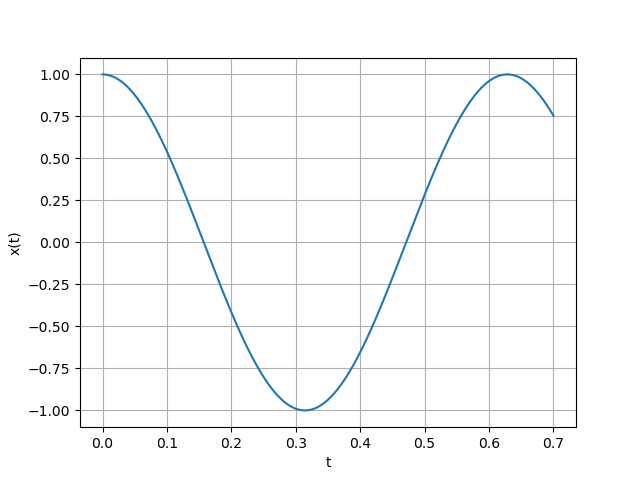
\includegraphics[width=\columnwidth]{Figure_1}
\end{center}
\caption{Plot of $x\brak{t}$}
\end{figure}
\end{document}
